\documentclass{beamer}
\usepackage{subfigure}
%\usetheme[left,width=80]{Marburg}
%\usetheme{Madrid}
%\usetheme{AnnArbor}
\usetheme{Antibes}
%\usetheme{Berkeley}
%\usetheme{Berlin}
\useinnertheme{rounded}
\usefonttheme{serif}
\setbeamertemplate{footline}[page number]{}
\setbeamertemplate{navigation symbols}{}
\title{CSE471 - Free and Open Source Software}
\author[Dayanand V]{Dayanand V \\ \texttt{v\_dayanand@cb.amrita.edu}}
\institute{Dept. of Computer Science and Engineering\\Amrita School of Engineering\\Amrita Vishwa Vidyapeetham}
\date{\today}
\AtBeginSection[]
{
	\begin{frame}<beamer>{Contents}
	\tableofcontents[currentsection,currentsubsection]
	\end{frame}
}
\begin{document}
\begin{frame}
	\titlepage
\end{frame}
\begin{frame}{Credits}
\textbf{The credits for the contents of this presentation goes to Karl Fogel and his book ``Producing Open Source Software". You are as free to reuse and redistribute the contents of this presentation as I am in using Fogel's book's content.}
\end{frame}
\section{Introduction}

\begin{frame}{Introduction}
\begin{itemize}
	\item About 90-95\% free software projects fail. Why?
	
	\begin{itemize}
		\item Unrealistic requirements
		\item Vague specifications
		\item Poor resource management
		\item Insufficient design phases
	\end{itemize}
	
	\item Aren't these the same reasons why closed-source projects fail?
	
	\begin{itemize}
		\item Yes, and there's more.
	\end{itemize}
	
	\item Sometimes, the developers do not appreciate the problems unique to open source development.  Like?
\end{itemize}
\end{frame}

\begin{frame}{Introduction}
	\begin{itemize}
	\item More reasons why open source projects fail.
	\begin{enumerate}
		\item Expecting hordes of oompa-loompas to magically volunteer for you.
		\item Expecting that releasing the source will be a cure of all its ills.
		\item Skimping on presentation and packaging to develop ``more important stuff".
		\item Expecting that the same management practices used for in-house development will work equally well on an open source project.
		\item Failures of ``Cultural Navigation".
	\end{enumerate}
	\end{itemize}
\begin{quote}
\tiny{``Open source does work, but it is most definitely not a panacea. If there's a cautionary tale here, it is that you can't take a dying project, sprinkle it with the magic pixie dust of ``open source," and have everything magically work out. Software is hard. The issues aren't that simple."
-Jamie Zawinski,  The Mozilla Project}
\end{quote}
\end{frame}

\section{History}

\begin{frame}{History}
\begin{itemize}
	\item At the dawn of commercial computers, `Software' sounded closer to an accessory than a business asset. 
	\item Customers (scientists, technicians etc) distributed patches to other customers and it was encouraged by the manufacturers. 
	\item There was no hardware standardization and the manufacturer wanted machine-specific code and knowledge to spread as widely as possible. 
	\item There was no Internet, and widespread frictionless sharing as we know it today, was not possible.
\end{itemize}
\end{frame}

\begin{frame}{The Rise of Proprietary Software and Free Software}
\begin{itemize}
	\item The advent of better `hardware' and 'high level' programming languages. 
	\item Selling software began looking like a good strategy. 
	\item If the user had freedom to modify the software and improve it, the `added value' patches would be of lesser significance. 
	\item Shared code can reach competitors. 
	\item Ironically, the Internet was getting off the ground around the same time.
\end{itemize}
\end{frame}

\begin{frame}{The Rise of Proprietary Software and Free Software - Conscious Resistance}
\begin{itemize}
	\item ``Richard Stallman" happened.
\end{itemize}
\begin{quote}
		\tiny{``We did not call our software "free software", because that term did not yet exist; but that is what it was. Whenever people from another university or a company wanted to port and use a program, we gladly let them. If you saw someone using an unfamiliar and interesting program, you could always ask to see the source code, so that you could read it, change it, or cannibalize parts of it to make a new program." -Richard Stallman}
\end{quote} 	
\begin{itemize}
	\item He went ahead and started the GNU Project and Free Software Foundation (FSF). 
	\item GNU was aimed at developing a completely free and open computer operating system and body of application s/w. 
	\item \small{``The GNU General Public License (GPL) says that the code may be copied and modified without restriction and that both copies and derivative works must be distributed \emph{under the same license as the original with no additional restrictions.}"}
\end{itemize}
\end{frame}

\begin{frame}{The Rise of Proprietary Software and Free Software - Conscious Resistance}
\begin{itemize}
	\item GNU slowly began gaining ground and was able to produce free replacements for many critical components of an OS. 
	\item GNU Emacs came into being. 
	\item The compiler collection GCC. 
	\item By 1990s, GNU had produced most parts of a free OS except for the kernel. 
	\item Linus Torvalds enters the scene with Linux, a kernel completed with the help of volunteers around the world. 
	\item Becomes GNU Linux, the world's first free and open source operating system.
\end{itemize}
\end{frame}

\begin{frame}{The Rise of Proprietary Software and Free Software - Accidental Resistance}
\begin{itemize}
	\item Berkeley Software Distribution (BSD) - University of California, Berkeley. 
	\item Non ideological practice of free software development. 
	\item X Window System developed at MIT allowed proprietary extensions over free software, but by itself was free. 
	\item \TeX , developed by Donald Knuth offering free publishing quality typesetting system was released open source with just some naming restrictions on derivatives. 
	\vspace{0.4cm} \\This presentation is built using `Beamer' which is an extension of \LaTeX , built on \TeX.
\end{itemize}
\end{frame}

\begin{frame}{Free Versus Open Source}
\begin{itemize}
	\item Free? As in \emph{free food}? 
	\item Free as in \emph{freedom}. 
	\item Freedom to share and modify the source code for any purpose.
	\item Case study : Battle of browsers (1990s), Netscaps vs IE.
	\item Free software - Morality vs Profitability.
	\item Conflict of opinion.
	\item 1998 - the word ``open source" is coined by Open Source Initiative (OSI 
\includegraphics[scale=0.1]{./Figures/index.png} ) to disambiguate ``free" and aimed at giving `free software' a good marketing.
\end{itemize}
\end{frame}

\begin{frame}{The Situation Today}
\begin{itemize}
	\item Free software has become a culture of choice.
	\item So what persuades all these people to stick together long enough to produce something useful? 
	\item The feeling that their connection to a project, and influence over it, is directly proportional to their contributions. 
	\item Clearly, projects with corporate sponsorship and/or salaried developers need to be especially careful in this regard.
\end{itemize}
\end{frame}

\section{Overview of the development process}

\begin{frame}{Look Around}
\begin{quote}
\tiny{``Every good work of software starts by scratching a developer's personal itch."\\ -Eric Raymond, `The Cathedral and the Bazaar'.}
\end{quote}
\begin{itemize}
	\item A good software results when the programmer has a personal interest in seeing the problem solved. 
	\item Today, we also have the phenomenon of organizations-for-profit, corporations, governments, non-profits, etc — starting large, centrally-conceived open source projects from scratch. 
	\item Case Study : Kuali Foundation 
	\item Identifying potential problems that are faced by a large community. 
	\item So, first, \emph{look around}! <github.com, openhub.net, sourceforge.net, directory.fsf.org>
\end{itemize}
\end{frame}

\begin{frame}{Start from What You Have}
\begin{itemize}
	\item Understanding clearly what the project is and what its not.
	\item Need for Documentation : Founders Vs New Comers.
	\item Investments : \emph{hacktivation energy}.
\end{itemize}
\end{frame}

\begin{frame}{Start from What You Have}
\begin{itemize}
	\item Choose a Good Name. 
	\begin{itemize}
		\item Gives an idea about what the project does.
		\item Easy to remember. 
		\item Good manners, good legal sense. 
		\item Getting top-level domains with forwarding to a central home site. 
		\item Handle availability in Twitter, FB.	
	\end{itemize}
\end{itemize}
\end{frame}

\begin{frame}{Start from What You Have}
\begin{itemize}
	\item Clear mission statement.
	\item State that the Project is `Free'. 
	\item A brief list of features and requirements.
\end{itemize}
\end{frame}

\begin{frame}{Start from What You Have}
\begin{itemize}
	\item Development Status 
	\begin{itemize}
		\item Should reflect reality.
		\item Alpha, Beta releases. 
		\item Availability for download. 
		\item Version Control and Bug Tracker Access. 
		\begin{itemize}
			\item GitHub.com - based on Git. 
			\item Rate of bug filing. 
		\end{itemize}
		\item Communication Channels
		\begin{itemize}
			\item Mailing List. 
			\item Chat room. 
			\item IRC Channel. 
		\end{itemize}
		\item Developer Guidelines. 
	\end{itemize}		
\end{itemize}
\end{frame}

\begin{frame}{Start from What You Have}
\begin{itemize}
	\item Documentation. 
	\begin{itemize}
		\item Minimal criteria: 
		\begin{itemize}
			\item Should tell the reader clearly how much technical expertise they're expected to have. 
			\item Tells clearly how to setup, and make sure that they've installed the software correctly. 
			\item Give one tutorial-style example of how to do a common task. 
			\item Label the areas where the documentation is known to be incomplete. 	
		\end{itemize}
		\item Developer documentation.	
	\end{itemize}
	\item Demos, Screenshots, Videos, and Example Output. 
	\item Hosting.
\end{itemize}
\end{frame}

\begin{frame}{Choosing a License and Applying It} 
\begin{itemize}
	\item The ``Do-Anything" licenses (MIT License). 
	\begin{itemize}
		\item Asserts nominal copyright (without actually restricting copying). 
		\item Code comes with no warranty. 
	\end{itemize}
	\item The GNU General Public License (GPL). 
	\begin{itemize}
		\item Translates loosely to - ``If you use my code, make sure you let others use yours."
	\end{itemize}
\end{itemize}
\end{frame}

\begin{frame}{Choosing a License and Applying It} 
\begin{itemize}
	\item Applying a license - Steps : 
	\begin{itemize}
		\item State the license clearly on the project's front page. 
		\item Put the full license text in a file called COPYING (or LICENSE) included with the source code. 
		\item Put a short notice in a comment at the top of each source file, naming :
		\begin{itemize}
			\item Copyright date
			\item Holder
			\item The kind of license
			\item Where to find the full text of the license. 
		\end{itemize}
	\end{itemize}
\end{itemize}
\end{frame}

\begin{frame}{Setting the Tone}
\begin{itemize}
	\item Avoid private discussions (1 $\langle$ n).
	\item Zero tolerance to rudeness. 
	\item Practice conspicuous code review. 
	\item Be open from day one! 
	\item Opening a formerly closed project. 
	\item Announcing. 
\end{itemize}
\end{frame}

\section{Technical Infrastructure}
\begin{frame}{Overview}
\begin{itemize}
	\item Website
	\item Mailing lists / Message forums
	\item Version control
	\item Bug tracking
	\item Real-time chat
\end{itemize}
\end{frame}

\begin{frame}{Version Control and Website}
\begin{itemize}
	\item Canned Hosting Services. 
	\item Github.com 
	\item Setting up a Github account. 
	\begin{enumerate} 
			\item Go to \emph{\href{https://github.com/}{https://github.com/}} 
			\item Sign up - Get yourself an account. 
			\item Go to \emph{\href{https://guides.github.com/activities/hello-world/}{https://guides.github.com/activities/hello-world/}} 
			\item Learn how to :
			\begin{enumerate}
				\item Create a `repository'.
				\item Open an `issue'.
				\item Create a `branch'.
				\item Make a `commit'.
				\item Open a `pull request'.
				\item `Merge' a pull request.
			\end{enumerate}
			\item Go to \emph{\href{https://pages.github.com/}{https://pages.github.com/}}  and follow the steps given there to setup a website for your project.
	\end{enumerate}
\end{itemize}
\end{frame}

\begin{frame}{Mailing list, Chat and Wiki}
\begin{itemize}
	\item Google groups. \emph{\href{https://groups.google.com}{https://www.groups.google.com}}
	\item Internet Relay Channel (IRC). \emph{\href{http://www.irchelp.org/irchelp/altircfaq.html}{http://www.irchelp.org/irchelp/altircfaq.html}}
	\item Mediawiki. \emph{\href{https://www.mediawiki.org}{https://www.mediawiki.org}}
\end{itemize}
\end{frame}

\section{Packaging, Releasing, and Daily Development}
\begin{frame}{Introduction}
\begin{itemize}
	\item Highway Repair analogy.	
	\item Mutually independent tasks are parallelized. 
	\item Release works can happen in parallel to development. 
\end{itemize}
\end{frame}

\begin{frame}{Releasing}
\begin{itemize}
	\item When does a release happen? 
	\begin{itemize}
		\item Some old bugs have been fixed  and new ones added. 
		\item New features added. 
		\item New configuration options might have been added, changing the installation procedure. 
		\item Incompatible changes might have been introduced. 
	\end{itemize}
\end{itemize}
\end{frame}

\begin{frame}{Releasing Numbering}
\begin{itemize}
	\item Unambiguously communicates the ordering of the release. 
	\item Indicates the degree and nature of the changes in the release. 
	\item Be consistent in choosing a numbering scheme, and stick with it. 
	\item Some examples would be:
	\begin{itemize}
		\item ``Project 1.2.3" 
		\item ``Project 1.2.3 (Alpha)" with the qualifier.
		\item ``Project 1.2.3 (Alpha 2)" with meta-qualifier.
	\end{itemize}
	\item Qualifiers : Alpha, Beta, Stable, Unstable, Development, and RC (for ``Release Candidate") etc.
	\item ``RC" always includes a numeric meta-qualifier, ``Project 1.2.3 (RC 1)" is possible, whereas ``Project 1.2.3 (RC)" is not. 		
\end{itemize}
\end{frame}

\begin{frame}{Releasing Numbering}
\begin{itemize}
	\item $\langle$ Project Name $\rangle$ $\langle$ Major Numbering $\rangle$.$\langle$ Minor Numbering$\rangle$. $\langle$ Micro Numbering$\rangle$ 
	\item ``Project 2.10.17" is the eighteenth micro release (or patch release) in the eleventh minor release line within the second major release series. 
\end{itemize}
\end{frame}

\begin{frame}{The Simple Strategy}
\begin{itemize}
	\item Adopted by \emph{\href{http://apr.apache.org/versioning.html}{APR project (Apache)}}. 
	\item Changes to the micro number only must be both forward- and backward-compatible. 
	\begin{itemize}
		\item Only bug fixes, or very small enhancements to existing features.
		\item No new features introduced in a micro release.
	\end{itemize}
	\item Changes to the minor number must be backward-compatible, but not necessarily forward-compatible. 
	\begin{itemize}
		\item New features can be introduced, but not too many.
	\end{itemize}
	\item Changes to the major number mark compatibility boundaries. A new major release can be forward- and backward-incompatible. 
	\begin{itemize}
		\item Entire new feature sets can be expected.
	\end{itemize}
\end{itemize}
\end{frame}

\begin{frame}{The Even/Odd Strategy}
\begin{itemize}
	\item Parity of the minor number defines stability of the software. 
	\item Even means stable, Odd means unstable. 
	\item Increments in the micro number still indicate bug fixes (no new features).  
	\item Increments in the major number still indicate big changes, new feature sets, etc. 
	\item Compatibility guidelines are still preserved.
\end{itemize}
\end{frame}

\begin{frame}{Release Branches}
\begin{itemize}
	\item The entire development tree will not be clean and ready for release at any time. 
	\item A release branch is just a branch in the version control system (see branch), on which the code destined for this release can be isolated from mainline 	development. 
	\item When a release branch is `stabilized', it is time to tag a snapshot (a micro release) from the branch. 
	\item `Stabilization' is the process of deciding which changes will be in the release, which will not, and shaping the branch content accordingly. 
	\item The `Release Owner' sets the release rules and has the final say in the case of any conflict.
	\item Voting on changes. 
	\item `Release Manager'.
\end{itemize}
\end{frame}

\begin{frame}{Packaging}
\begin{itemize}
	\item Free software is distributed as source code or pre-built binary packages.
	\item Shipping formats:
	\begin{itemize}
		\item *nix OSes - TAR compressed by /emph{compress, gzip, bzip, or bzip2}. 
		\item MS Windows - /emph{zip} format. 
	\end{itemize}
	\item Name of the package contains the software's name plus the release number, plus the format suffixes appropriate for the archive type.
\end{itemize}
\end{frame}

\begin{frame}{Layout}
\begin{itemize}
	\item Once uncompressed, the root directory should contain:
	\begin{itemize}
		\item A `README' plain text file describing :
			\begin{itemize}
				\item what the software does.
				\item what release this is.
				\item link to the project's website etc.
			\end{itemize}
		\item An `INSTALL' file giving instructions on how to build and install the software for all supporting operating systems.
		\item A COPYING or LICENSE file, giving the software's terms of distribution. 
		\item A CHANGES file (sometimes called NEWS), explaining what's new in this release.
	\end{itemize}
\end{itemize}
\end{frame}

\begin{frame}{Compilation and Installation}
\begin{itemize}
	\item For compiled languages, in *NIX systems, the installation procedure of tarred source code typically would be like: 
	\begin{itemize}
		\item \$ ./configure (auto-detects the environment and and prepares the build process)
		\item \$ make (builds the software)
		\item \$ make install (installs the software on the system)
	\end{itemize}
	\item Installation of binary packages:
	\begin{itemize}
		\item RPM system for RedHat GNU/Linux distros. 
		\item APT system for Debian GNU/Linux distros. 
	\end{itemize}
\end{itemize}
\end{frame}

\begin{frame}{Testing}
\begin{itemize}
	\item Regression testing + Manual Testing. 
	\item Once all check-list criteria are met, the packages are digitally signed using \emph{\href{http://www.gnupg.org/}{GnuPG}} or \emph{\href{http://www.pgpi.org/}{PGP}} etc. 
	\item Once approved, the release should be placed into the project's download area, accompanied by the digital signatures, and by MD5/SHA1 checksums.
	\item The purpose of all this signing and checksumming is to give users a way to verify that the copy they receive has not been maliciously tampered with.
\end{itemize}
\end{frame}

\begin{frame}{Candidate Releases}
\begin{itemize}
	\item Remember the qualifier `RC'? 
	\item Candidates releases are put out first before official release of a new version. 
	\item The aim is to subject the code to wide testing before blessing it as an official release. 
	\item If problems are found, they are fixed on the release branch and a new candidate release is rolled out. 
	\item If there are no unacceptable bugs left, the last candidate release becomes the official release.
\end{itemize}
\end{frame}

\begin{frame}{Announcing Releases}
\begin{itemize}
	\item The announcement should include:
	\begin{itemize}
		\item The URL to the downloadable release tarball ahouls always be accompanied with the MD5/SHA1 checksums and pointers to the digital signatures file. 
		\begin{itemize}
			\item Announcing in multiple forums/mailing lists.
			\item Reassurance on security.
		\end{itemize} 
		\item The relevant portion of the CHANGES file. 
		\item Credits where it is due.
	\end{itemize}
\end{itemize}
\end{frame}

\begin{frame}{Maintaining Multiple Release Lines}
\begin{itemize}
	\item Most mature projects maintain multiple release lines in parallel. 
	\item After 1.0.0 comes out, that line should continue with micro (bugfix) releases 1.0.1, 1.0.2, etc., until the project explicitly decides to end the line.
	\item Announcing the `end of life' of release. 
	\item Some projects set a window of time during which they pledge to support the previous release line. 
	\item Some projects waits for the bug reports percentage to drops below a certain point to stop support. 
	\item For each release, make sure to have a target version or target milestone available in the bug tracker, so people filing bugs will be able to do so against the proper release.
\end{itemize}
\end{frame}

\begin{frame}{Security Releases}
\begin{itemize}
	\item A security release is a release made SOLELY to close a security vulnerability. 
	\item This is friendly to the administrators who may need to deploy the security fix, but whose upgrade policy stipulates that they not deploy any other changes at the same time. 
	\item An extra component can be added to an existing release to indicate that it contains only security changes (Eg: 1.1.2.1).
\end{itemize}
\end{frame}

\begin{frame}{Releases and Daily Development}
\begin{itemize}
	\item Release Stabilization. 
	\item Have each commit to be a single logical change, and don't mix unrelated changes in the same commit. 
	\item If a change is too big or too disruptive to do in one commit, break it across N commits. 
	\item Each commit is a well-partitioned subset of the overall change, and includes nothing unrelated to the overall change.
\end{itemize}
\end{frame}

\begin{frame}{Planning Releases}
\begin{itemize}
	\item Deadlines, Schedules. 
	\item Discussions, Compromises. 
	\item Depending on the complexity of the release process, and the nature of the project, somewhere between every three and six months is usually about the right gap between releases. 
	\item Maintenance lines may put out micro releases a bit faster, if there is demand for them. 
\end{itemize}
\end{frame}

\section{Licenses, Copyrights and Patents}
\begin{frame}{Aspects of Licenses}
\begin{itemize}
	\item Differences between licenses boil down to a few often recurring issues :
	\begin{itemize}
		\item Compatibility with proprietary licenses. 
		\item Compatibility with other types of free licenses. 
		\item Enforcement of crediting. 
		\item Protection of trademark. 
		\item Patent snapback. 
		\item Protection of ``artistic integrity". 
	\end{itemize}	
\end{itemize}
\end{frame}

\begin{frame}{GPL and License Compatibility}
\begin{itemize}
	\item GPL Requirements:
	\begin{itemize}
		\item  Any derivative work must itself be distributed under the GPL.
		\item No additional restrictions may be placed on the redistribution of either the original work or a derivative work. 
	\end{itemize}
	\item Incompatibilities: 
	\begin{itemize}
		\item Credit enforcement as a new policy cannot be applied on a GPL licensed code. 
	\end{itemize}
	\item Free Software Foundation maintains a \emph{\href{http://www.gnu.org/licenses/license-list.html}{list}} showing which licenses are compatible with the GPL and which are not.
\end{itemize}
\end{frame}

\begin{frame}{Choosing a License}
\begin{itemize}
	\item Use one of the widely-used, well-recognized existing licenses. 
	\item Advantages:
	\begin{itemize}
		\item People won't feel they have to read the legalese in order to use your code, because they will have already done so for that license a long time ago. 
		\item They are the products of much thought and experience and the modern versions represent a great deal of accumulated legal and technical wisdom.
	\end{itemize}
\end{itemize}
\end{frame}

\begin{frame}{Choosing a License}
\begin{itemize}
	\item A list of licenses that meet the criteria: \footnote{\textbf{\tiny{Assignment \#3 : Study in detail and submit a report about the differences between the above licenses (with a clear tabular column) and where they would deem best to be used.}}}
	\begin{itemize}
		\item \emph{\href{http://www.gnu.org/licenses/gpl.html}{\alert{GNU General Public License version 3 (GPL-3.0)}}}
		\item \emph{\href{http://www.gnu.org/licenses/agpl.html}{\alert{GNU Affero General Public License version 3 (AGPL-3.0)}}}
		\item \emph{\href{https://www.mozilla.org/MPL/}{Mozilla Public License 2.0 (MPL-2.0)}}
		\item \emph{\href{http://www.gnu.org/licenses/lgpl.html}{GNU Library or ``Lesser" General Public License version 3 (LGPL-3.0)}}
		\item \emph{\href{https://www.eclipse.org/legal/epl-v10.html}{Eclipse Public License 1.0 (EPL-1.0)}}
		\item \emph{\href{http://opensource.org/licenses/MIT}{\alert{MIT license (MIT)}}}
		\item \emph{\href{http://apache.org/licenses/LICENSE-2.0}{Apache License 2.0 (Apache-2.0)}}
		\item \emph{\href{http://opensource.org/licenses/BSD-2-Clause}{BSD 2-Clause (``Simplified" or ``FreeBSD") license}}	
	\end{itemize}
\end{itemize}
\end{frame}
	
\begin{frame}{Contributor Agreements}
\begin{itemize}
	\item Handling copyright ownership for free code and documentation that were contributed to by many people: 
	\begin{enumerate}
		\item Ignore the issue of copyright entirely. 
		\item Collect a contributor license agreement (CLA) from each person who works on the project, explicitly granting the project the right to use that person's contributions.
		\item Get actual copyright assignment (CA from contributors, so that the project (i.e., some legal entity, usually a nonprofit) is the copyright owner for everything.
	\end{enumerate}
	\item Even under centralized copyright ownership, the code remains free, because open source licenses do not give the copyright holder the right to retroactively proprietize all copies of the code.
\end{itemize}
\end{frame}

\begin{frame}{\emph {\href{http://developercertificate.org}{Developer Certificates of Origin (DCO)}}}
\begin{itemize}
	\item An attestation that the contributor intends to contribute the enclosed code under the project's license, and that the contributor has the right to do so.
	\item The contributor indicates her understanding of the DCO once, early on, for example by emailing its text from her usual contribution address to a special archive at the project.
	\item The contributor includes a ``Signed-Off-By:" line in her patches or commits, using the same identity, to indicate that the corresponding contribution is certified under the DCO.
	\item The DCO relies on the project's native open source license for any trademark or patent provisions, which in most cases is fine.
\end{itemize}
\end{frame}

\begin{frame}{Proprietary Re-licensing}
\begin{itemize}
	\item An open source version of the software is available under the usual open source terms, while a proprietary version is available for a fee.
	\item Two types:
	\begin{enumerate}
		\item Selling exceptions to copyleft requirements. 
		\begin{itemize}
			\item Sells users a promise to not enforce the redistribution requirements of the open source version's license.
			\item Eg:- MySQL Database Engine. GPL v2. 
		\end{itemize}
		\item The freemium or open core model. 
		\begin{itemize}
			\item Uses an open source version to drive sales of a presumably fancier proprietary version. 
		\end{itemize}
	\end{enumerate}
	\item The catch here is that GPL's terms are something the copyright holder imposes on everyone else; the owner is therefore free to decide not to apply those terms to itself.
\end{itemize}
\end{frame}

\begin{frame}{Proprietary Re-licensing}
\begin{itemize}
	\item Problems with proprietary re-licensing:
	\begin{enumerate}
		\item Discourages the normal dynamics of open source projects. 
		\item Any code contributors from outside the company are now effectively contributing to two distinct entities, one which they usually do not prefer. 
		\item there is a deep motivational problem for open source projects that operate in the shadow of a proprietarily re-licensed version. 
		\item Hybrid ``shakedown" models: anyone who makes commercially significant use of the code ends up being pressured to purchase a proprietary license as a way of protecting their commercial revenue stream from harassment.
	\end{enumerate}
\end{itemize}
\end{frame}
	
\begin{frame}
\begin{itemize}
	\item A trademarked name or symbol is a way for an entity (who owns or controls that trademark), to signal, in an easily recognizable way, that they approve of a particular product. 
	\item Trademarks do not restrict copying, modification, or redistribution. 
	\item Trademark is unrelated to copyright, and does not govern the same actions that copyright governs.
	\item Case study: Mozilla Firefox, the Debian Project, and Iceweasel.
	\item Case study: The GNOME Logo and the Fish Pedicure Shop.
\end{itemize}
\end{frame}

\begin{frame}{Patents}
\begin{itemize}
	\item The only real threat against which the free software community cannot defend itself. 
	\item Once someone has accused a free software project of infringing a patent, the project must either stop implementing that particular feature, or expose the project and its users to expensive and time-consuming lawsuits. 
	\item Modern free software licenses generally have clauses to combat, or at least mitigate, the dangers arising from software patents.
	\item Usually these clauses work by automatically revoking the overall open source license for any party who makes a patent infringement claim based on either the work as a whole, or based on the claimant's code contributions to the project. 
\end{itemize}
\end{frame}

\section{Introduction to GNU Autotools}
\begin{frame}{Introduction to GNU Autotools}\pause
\begin{itemize}
	\item Outcome of the demand for a de-facto standard for compiling and installing software.\pause
	\item Autoconf, Automake, and Libtool were developed separately, to make tackling the problem of software configuration more manageable by partitioning it. \pause
	\item By-products of the GNU/Linux project.
	\end{itemize}
\end{frame}

\begin{frame}{GNU Autotools and what they do!}
\begin{itemize}
	\item Autoconf:\pause
	\begin{itemize}
		\item A tool that makes your packages more portable by performing tests to discover system characteristics before the package is compiled. \pause
		\item The source code adapts to these differences. \pause
	\end{itemize}
	\item Automake:\pause
	\begin{itemize}
		\item A tool for generating `Makefile's--descriptions of what to build--that conform to a number of standards. \pause	 
		\item It substantially simplifies the process of describing the organization of a package. \pause
		\item Performs additional functions such as dependency tracking between source files. \pause
	\end{itemize}
	\item Libtool:\pause
	\begin{itemize}
		\item A command line interface to the compiler and linker that makes it easy to portably generate static and shared libraries, regardless of the platform it is running on.
	\end{itemize}
\end{itemize}
\end{frame}

\begin{frame}{History of Autotools}
\begin{itemize}
	\item The advent and popularity of Unix. \pause
	\item POSIX standards. \pause
	\item Need for an organized approach to handle the differences.\pause
	\item Earlier tools :\pause
	\begin{itemize}
		\item The Metaconfig program, by Larry Wall, Harlan Stenn, and Raphael Manfredi.
    	\item The Cygnus `configure' script, by K. Richard Pixley, and the original GCC `configure' script, by Richard Stallman.
		\item The GNU Autoconf package, by David MacKenzie.
		\item Imake, part of the X Window system. 
	\end{itemize}\pause
	\item All these tools had a \emph{configuration step} and a \emph{build step}.\pause
	\item The configuration step would generate `Makefile's, and perhaps other files, which would then be used during the build step using the `make' command. \pause
	\item The use of `feature tests' made software compatible across OS variants without change in source code.
\end{itemize}
\end{frame}

\begin{frame}{History of Autotools}
\begin{itemize}
	\item By 1994, Autoconf was a solid framework for handling the differences between Unix variants. But, \pause
	\begin{itemize}
		\item Program developers still had to write large `Makefile.in' files in order to use it.\pause
		\item The `configure' script generated by autoconf would transform the `Makefile.in' file into a `Makefile' used by the make program. \pause
	\end{itemize}	
\end{itemize}
\end{frame}

\begin{frame}{History of Autotools}
\begin{itemize}
	\item Since most programs are built in much the same way, there was a great deal of duplication in `Makefile.in' files.\pause
	\item Also, the GNU project developed a reasonably complex set of standards for `Makefile's, and it was easy to get some of the details wrong.\pause
	\item These factors led to the development of Automake.\pause
	\begin{itemize}
		\item The developer writes files named `Makefile.am'; these use a simpler syntax than ordinary `Makefile's. automake reads the `Makefile.am' files and produces `Makefile.in' files. \pause
		\item A script generated by autoconf converts these `Makefile.in' files into `Makefile's. \pause
		\item  automake also adds any rules required by the GNU `Makefile' standards. \pause
	\end{itemize}
\end{itemize}
\end{frame}


\begin{frame}{History of Autotools}
\begin{itemize}
	\item Unix added support for shared libraries.\pause
	\item Advantages of using shared libraries. \pause
	\item Development of Libtool began. \pause
	\begin{itemize}
		\item Libtool is a collection of shell scripts which handle the differences between shared library generation and use on different systems. 
		\item It is closely tied to Automake, although it is possible to use it independently. 
	\end{itemize}
	\item Over time, Libtool has been enhanced to support more Unix variants and to provide an interface for standardizing shared library features. 
\end{itemize}
\end{frame}

\begin{frame}{History of Autotools}
\begin{itemize}
	\item In 1995, Microsoft released Windows 95 which became widely popular.\pause
	\item Autoconf and Libtool provided a framework to support portability (from a single source code base) to Windows as well.\pause
	\item To support this, the GNU bash shell was ported to Windows as Cygwin which implements the basic Unix API in Windows. \pause
	\item Autoconf and Libtool support Windows directly, using either the Cygwin interface or the Visual C++ tools from Microsoft.\pause
	\item Automake has also been ported to Windows but it requires Perl to be installed.
\end{itemize}
\end{frame}

\begin{frame}{Running `configure'}
\begin{itemize}
	\item Command line options.
	\begin{itemize}
		\item \emph{\tiny{\href{https://www.sourceware.org/autobook/autobook/autobook\_14.html\#Configuring}{https://www.sourceware.org/autobook/autobook/autobook\_14.html\#Configuring}}}\pause
		\item `-\hspace*{0.01cm}-cache-file=file' \pause
		\item `-\hspace*{0.01cm}-help' \pause
		\item `-\hspace*{0.01cm}-quiet' or `-\hspace*{0.01cm}-silent' \pause
		\item `-\hspace*{0.01cm}-disable-$\langle$feature$\rangle$' \pause	
		\item `-\hspace*{0.01cm}-enable-feature[=arg]'etc..
	\end{itemize}
	\item Source tree, Build tree and Install tree.
\end{itemize}
\end{frame}

\begin{frame}{Files generated by configure}
\begin{itemize}
	\item `config.cache'\pause
	\item `config.log'\pause
	\item `config.status'\pause
	\item `config.h'\pause
	\item `Makefile'\pause
\end{itemize}
\end{frame}

\begin{frame}{Makefiles and targets}
\begin{itemize}
	\item Makefiles contain specifications of dependencies between files and how to resolve those dependencies
	\item Targets - the task to be performed by the Makefile:
	\begin{itemize}
		\item make \emph{all}
		\item make \emph{check}
		\item make \emph{install}
		\item make \emph{clean} etc.
	\end{itemize}
\end{itemize}
\end{frame}

\begin{frame}{Make files}
\begin{itemize}
	\item The `make' program attempts to bring a target up to date by bring all of the target's dependencies up to date (the dependent has a more recent timestamp than the target).
	\item Dependencies and dependency graph.	
	\begin{figure}
		\subfigure[Makefile]{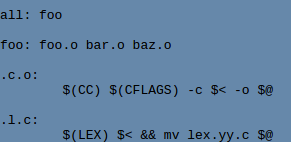
\includegraphics[scale=0.42]{./Figures/MakefileExample.png}}
		\subfigure[Dependency Graph]{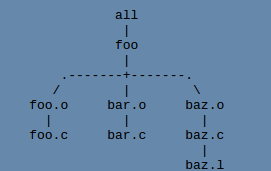
\includegraphics[scale=0.35] {./Figures/MakefileDependencyGraphExample.png}}
%		\caption{Examples}
	\end{figure}
	\item When leaf nodes are found in the dependency graph, the `Makefile' must include a set of shell commands to bring the dependent up to date with the dependency.
\end{itemize}
\end{frame}

\begin{frame}{Makefiles}
\begin{itemize}
	\item Each of the shell commands are run in their own sub-shell and, unless the `Makefile' instructs make otherwise.
	\item Each command must exit with an exit code of 0 to indicate success.
	\item Target rules can be written which are executed unconditionally (by specifying that the target has no dependents).
	
\end{itemize}
\end{frame}

\begin{frame}{Writing Makefiles}
\begin{itemize}
	\item Syntax:
	\begin{figure}
		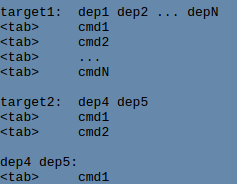
\includegraphics[scale=0.4]{./Figures/MakefileSyntax.png}
	\end{figure}
	\item Command prefixes - `@', `-'
	\item Macros
	\begin{itemize}
		\item Starts with a dollar sign. 
		\item Eg:- \$CC
		\item Define a make variable using a `var=value' syntax: `CC = ec++' (Default value of \$CC is `cc')
		\item  `\$@' and `\$$\langle$' represent the names of the target and the first dependency for the rule in which they appear
	\end{itemize}
\end{itemize}
\end{frame}

\begin{frame}{Writing Makefiles}
\begin{itemize}
	\item Example:
	\begin{figure}
		\subfigure[File] {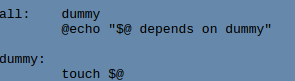
\includegraphics[scale=0.45]{./Figures/MacroExampleFile.png}}
		\subfigure[Output] {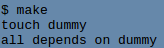
\includegraphics[scale=0.5]{./Figures/MacroExampleOutput.png}}
	\end{figure}
	\item Suffix Rules: wildcard pattern that can match targets
	\item Example:
	\begin{figure}
		
\includegraphics[scale=0.4]{./Figures/SuffixRulesExample.png}
	\end{figure}
	\item This rule will match any target that ends in `.o' and are said to always be dependent on `.c'
\end{itemize}
\end{frame}

\end{document}